\documentclass[11pt]{amsart}
\usepackage[colorlinks=true]{hyperref}
\usepackage{graphicx}
\usepackage{float}
\usepackage{listings}


\title{An API for Economic Agents}
\author{David R. Pugh, Daniel F. Tang, J. Doyne Farmer}
\date{\today}

\begin{document}
\maketitle

\section{Motivation...}
Our objective is to create a \textit{user-friendly} toolkit for building \textit{scalable}, \textit{data-driven} agent-based models (ABMs) of \textit{economic} systems.

\subsection{Requirements}

\section{Implementation}
\begin{figure}[H]
\centering
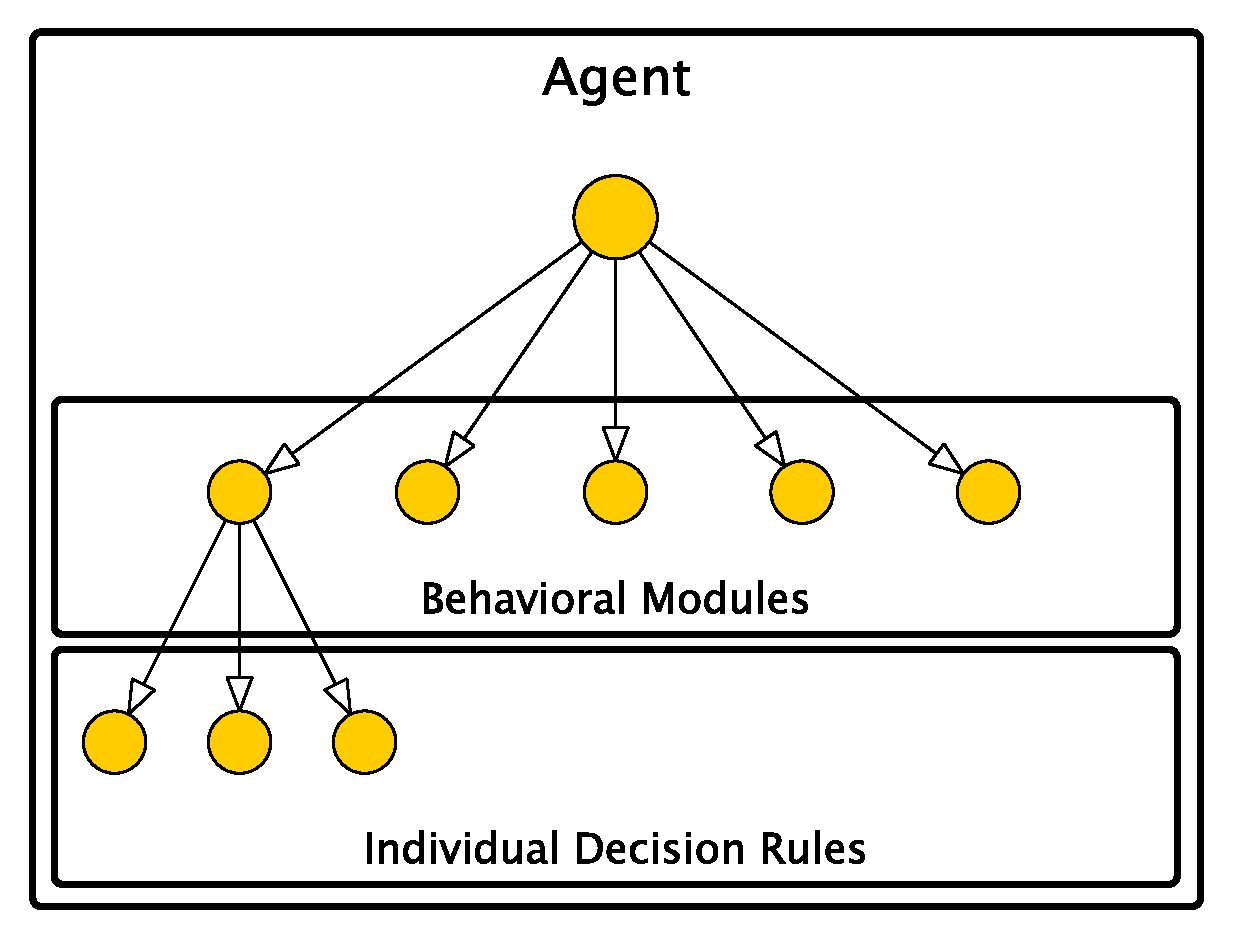
\includegraphics[width=10cm]{hierarchical-actor.pdf}
\caption{An economic actor in our framework is represented as a hierarchical tree of Akka Actors.}
\end{figure}

\section{Model Layer}
An economy is populated with many seemingly disparate types of agents (i.e., consumers, producers, financiers, government, etc).  Our goal is to distill the core essence (in terms of data and behaviors) of these different agents into a multi-layered Application Programming Interface (API) defining a generic \textit{economic agent} that can then be specialized to the various types of economic agents needed for any particular model.

Several key features distinguish \textit{economic} agents from more generic types of agents. At a minimum these features include: purpose driven (or goal oriented) behaviour, an ability to learn, and the ability to anticipate future events. This suggests that our framework will need APIs for...
\begin{itemize}
    \item Goals or objectives (and their associated behavioral rules): Our goals/objectives API needs to be as un-opinionated as possible as prospective users of ScalABM are likely to have strong opinions on how to define appropriate goals and decision rules for their agents. At the same time, we will need to have some type of underlying null model of agent goals/objectives. Utility maximization, Belief-Desire-Intent (BDI), probabilistic discrete choice (AKA, random utility maximization) are possibilities. These frameworks seem to have much in common.  
    \item Learning rules: A large number of various learning rules/mechanisms have been proposed in the academic literature. Roughly, learning rules seem to fall into two camps: learning through previous experience (i.e., reinforcement learning) and learning through observation (i.e., belief learning). Useful references for learning rules for ABMs are the two handbook chapters \href{http://web.uvic.ca/~mingkang/econ353/project/Brenner.pdf}{Brenner (2006)} and \href{http://www.socsci.uci.edu/~duffy/papers/duffy2006.pdf}{Duffy (2006)}.
    \item Expectations formation rules: A large number of various expectation formation rules have been proposed in the literature. Useful references for expectation formation rules are \href{http://feb.kuleuven.be/fac/Slides_Degrauwe/HomHBchapter23.pdf}{Hommes (2006)}, \href{http://econ.columbia.edu/files/econ/content/hommes_background_material_2.pdf}{Anufriev and Hommes (2012)}, \href{http://www.columbia.edu/~mw2230/AREcon.pdf}{Woodford (2013)}, \href{http://www.emeraldinsight.com/doi/pdfplus/10.1108/S0193-230620140000017002}{Assenza et al (2014)}.
    \item Decision rules: Depending on type, an economic agent might need to make a number of supply or demand decisions.
\end{itemize}

Concurrent communication between real economic agents is a fundamental fact of economic life. While a substantial amount of communication between economic agents is direct (or ``peer-to-peer''), perhaps the majority of communication between agents is indirect via market institutions. Our framework leverages the Actor model of concurrency (as implemented in Akka) to model both direct and indirect communication between economic agents via concurrent asynchronous message passing.

This suggests that our framework will need APIs for...
\begin{itemize}
    \item Communications: In order to constrain the communication problem, we need to develop an API that defines both the type and the content of messages that can be passed between agents. Our agent communication API is influenced by, but not slave to, the \href{http://www.fipa.org/}{Foundation for Intelligent Physical Agents (FIPA)} compliant \href{http://www.fipa.org/specs/fipa00037/SC00037J.pdf}{Agent Communication Language (ACL)}. 
    \item Market institutions: In addition to being able to communicate with economic agents, a market needs to have an auction mechanism for determining prices and quantities (i.e., double-auction mechanism, market clearing, etc) and a market needs to have a clearing mechanism for processing transactions (although this might simply involve linking to some underlying payment system).
\end{itemize}

\subsection{An API for agent communication}
Concurrent communication between real economic agents is a fundamental fact of economic life. While a substantial amount of communication between economic agents is direct (or ``peer-to-peer'') the majority of communication between agents is indirect via market institutions.  

We have developed an API for agent communication which specifies:
\begin{itemize}
    \item a set of abstract message types that impose structure on the messages passed between a group of economic agents,
    \item a set of abstract protocols that impose structure on conversations (i.e., sequences of messages) between a group of economic agents. 
\end{itemize}
Each abstract message type can be thought of as defining an ``envelope'' containing the actual content of the message that is to be exchanged between a group of economic agents. Defining envelopes containing messages is useful because it allows agents to react based on the type message received. Each abstract protocol defines a particular subset of message types that can be sent by an agent in response to a particular type of message that it has received. 

Our agent communication API is influenced by, but not slave to, the \href{http://www.fipa.org/}{Foundation for Intelligent Physical Agents (FIPA)} compliant \href{http://www.fipa.org/specs/fipa00037/SC00037J.pdf}{Agent Communication Language (ACL)}.

\subsubsection{Examples}
An important example of an abstract message type is the \texttt{RequestLike} message. In our agent communication API this abstract message has three concrete types:
\begin{itemize}
    \item \texttt{Request}: Agent (i.e., \texttt{sender}) sends a \texttt{Request} message to another agent (i.e, \texttt{receiver}) if the \texttt{sender} wants the \texttt{receiver} to perform some action as specified in the message content.
    \item \texttt{RequestWhen}: Agent (i.e., \texttt{sender}) sends a \texttt{RequestWhen} message to another agent (i.e, \texttt{receiver}) if the \texttt{sender} wants the \texttt{receiver} to perform some action as specified in the message content when some precondition is satisfied.
    \item \texttt{RequestWhenever}: Agent (i.e., \texttt{sender}) sends a \texttt{RequestWhenever} message to another agent (i.e, \texttt{receiver}) if the \texttt{sender} wants the \texttt{receiver} to perform some action as specified in the message content whenever some precondition is satisfied.
\end{itemize}

Another important abstract message type is the \texttt{ResponseLike} message. In our agent communication API this abstract message has two concrete types:
\begin{itemize}
    \item \texttt{Agree}: A message sent from some agent (i.e., \texttt{sender}) to another agent (i.e., \texttt{receiver}) indicating that the sender has agreed to perform some action(s) as specified in a \texttt{RequestLike} message previously sent by the \texttt{receiver}. 
    \item \texttt{Refuse}: A message sent from some agent (i.e., \texttt{sender}) to another agent (i.e., \texttt{receiver}) indicating that the sender has refused a \texttt{RequestLike} message.
\end{itemize}

Finally consider four additional message types:
\begin{itemize}
    \item \texttt{Inform}: A message sent from some agent (i.e., sender) to another agent (i.e., receiver) informing the receiver that some proposition is true.
    \item \texttt{NotUnderstand}: A message sent from some agent (i.e., sender) to to another agent (i.e., recevier) informing it that some previously received message was not understood.
    \item \texttt{Cancel}: A message sent from some agent (i.e., sender) to another agent (i.e., receiver) indicating that a previously received Request message (i.e., request) to perform some action should be canceled.
    \item \texttt{Failure}: A message sent from some CommunicatingActor (i.e., sender) to another agent (i.e., receiver) indicating that some action was attempted, but that the attempt failed.
\end{itemize}

With these message types in hand, we define a \texttt{RequestHandler} protocol that specifies a valid sequences of these message types (i.e., a ``request conversation'').
\begin{enumerate}
    \item An agent (i.e., \texttt{initiator}) sends a \texttt{RequestLike} message to another agent (i.e., \texttt{participant}).
    \item The \texttt{participant} responds with either an \texttt{Agree} or \texttt{Refuse} message (or in extreme cases with a \texttt{NotUnderstood} message).
    \item Assuming the \texttt{participant} agreed to the request, the \texttt{participant} attempts to perform necessary actions and then responds with either \texttt{Failure} or \texttt{Inform}, depending.
\end{enumerate}

There is an important exception to the protocol. At any point the \texttt{initiator} of the request can send a \texttt{Cancel} message to the \texttt{participant} indicating that it wishes to \texttt{cancel} its previous request.

Examples of additional abstract communication protocols can be found on the \href{http://www.fipa.org/repository/standardspecs.html}{FIPA} web site. Concrete implementations of these abstract protocols will define behavioral strategies that will be mixed together to create an specific economic agent.

% The elements that distinguish {\it economic agents} are:
% \begin{itemize}
%     \item balance sheets
%     \item expectations
%     \item objective functions
%     \item decision rules (i.e., functions the specify actions, which are typically based on objective functions and expectations, and possibly other factors)
%     \item interaction with markets
%     \item direct interactions with each other, e.g. in negotiation.
% \end{itemize}
% We do not mean to imply that all economic agents will have all of these elements.  There are, for example, many examples of economic agents who have no direct interactions with each other.  We also do not mean for this list to be exclusive.  This list simply contains elements shared by many economic agents.  Examples of economic agents are households, firms, and banks (which may or may not be treated as a type of firm).

% For example, consider households.  Households have a balance sheet whose most important elements might be a house, a bank account, and perhaps mutual fund investments.  The household will form expectations about factors such as future earnings or housing prices.  It will interact with the labor market and possibly with financial markets or housing markets.  It may or may not make sense to use some form of utility maximization. 

% The treatment of firms in an ABM can vary from a bare-bones finance model that represents a firm as an exogenous source of dividends, to a more articulated model that includes the goods produced by the firm, the workers employed by the firm (and the wages paid to them), the production function of the firm, etc.  




% We need to have some notion of contracts that connect various economic actors. Ideally contracts should be composable so that it is easy to create more sophisticated contracts out of simple building blocks.  We ideally want this to be set up so that agents more or less automatically obey the terms of their contracts, except when they don't, when things may get more complicated.  Mechanisms such as default resolution are essential.

% Finally, we want to have a standard toolkit providing a menu of different ways for actors to form exceptions and make decisions, such as BDI, probabilistic discrete choice, or Experience Weighted Attraction.  ({\it Not sure about the right way to slice this one}). 



% In order to implement an economy we find it useful to organize the functions described above in a more abstract manner.  
% \begin{figure}[ht]
% 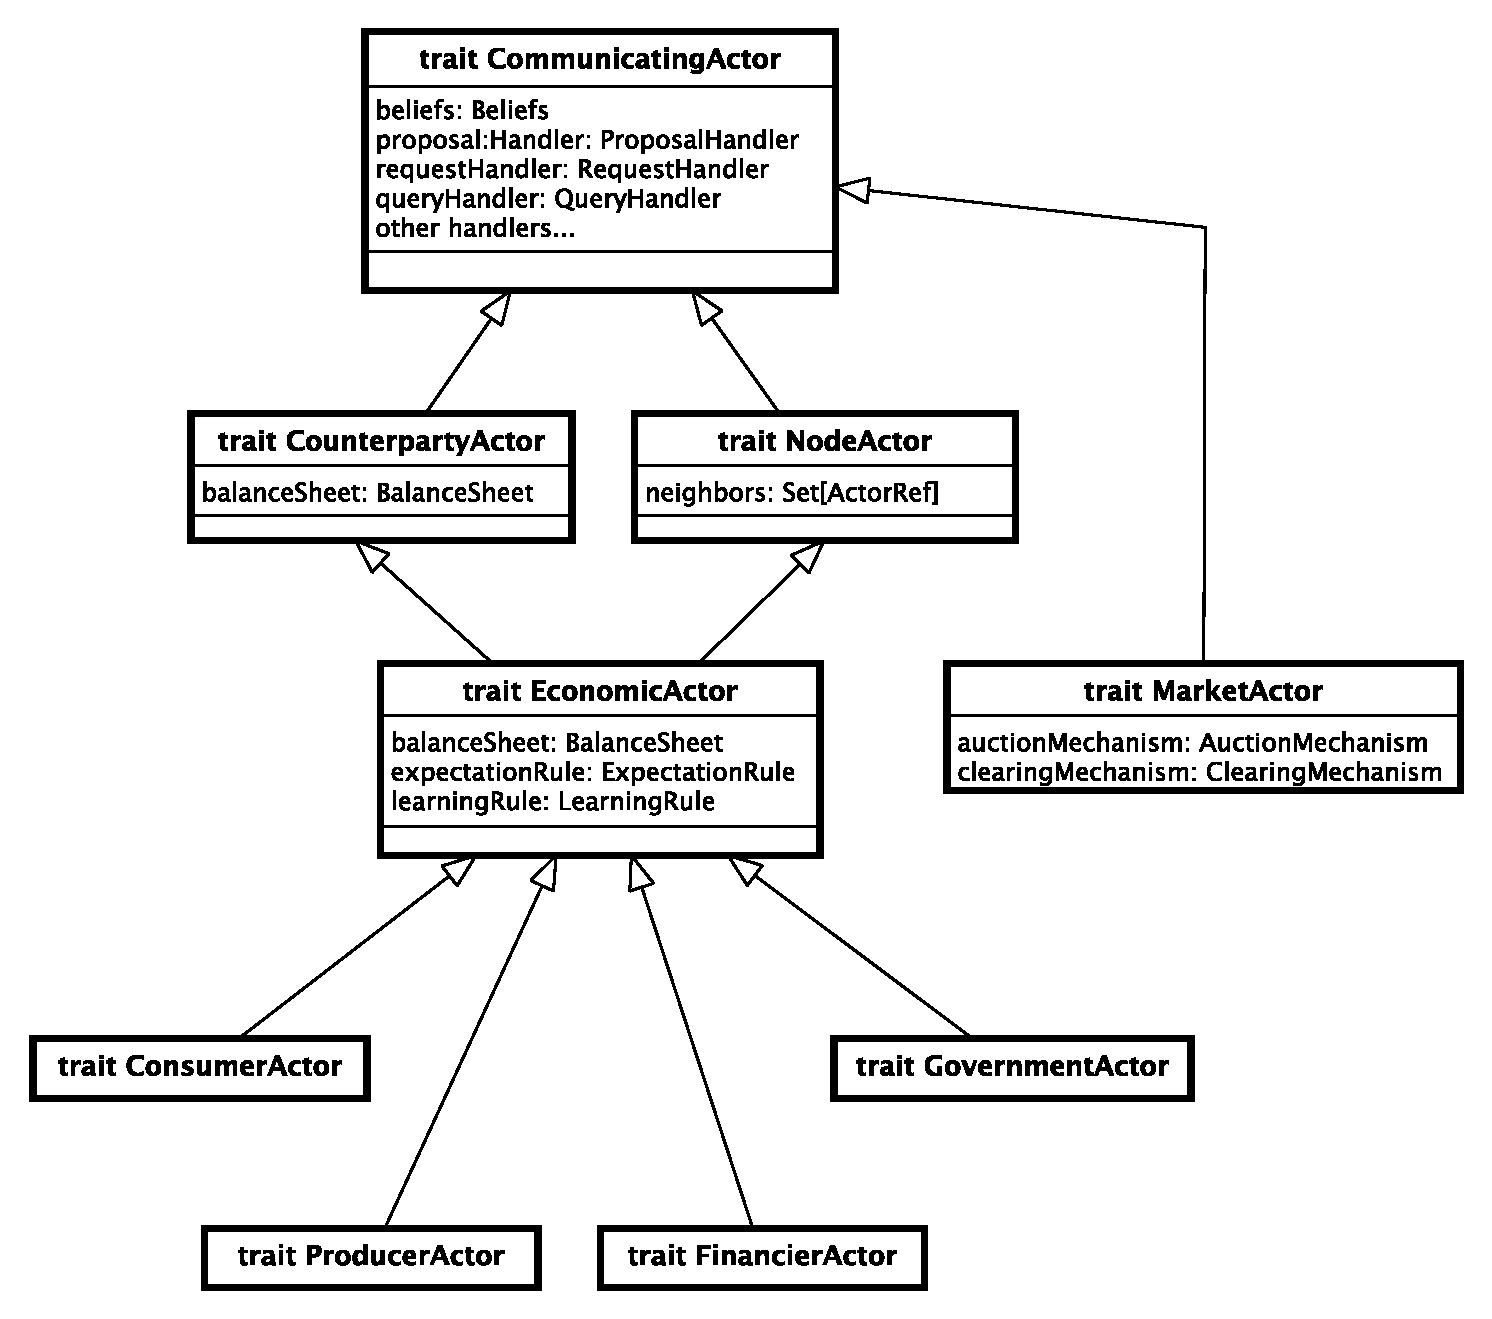
\includegraphics[scale=0.4]{class-diagram.pdf}
% \end{figure}

% Quick list of current requirements for an \texttt{EconomicActor}:
% \begin{itemize}
%     \item an \texttt{EconomicActor} is a \texttt{CommunicatingActor},
%     \item an \texttt{EconomicActor} is a \texttt{CounterpartyActor},
%     \item an \texttt{EconomicActor} is a \texttt{NodeActor} in some multi-plex network.
%     \item an \texttt{EconomicActor} has a collection of \texttt{PrivateInformation},
%     \item an \texttt{EconomicActor} has a collection of \texttt{PublicInformation}.
%     \item an \texttt{EconomicActor} should be able to form expectations about the future,
%     \item an \texttt{EconomicActor} should be able to learn about its economic environment and adapt its behavior.
% \end{itemize}

% Below we outline the APIs describing a \texttt{CounterpartyActor}, \texttt{CommunicatingActor}, and \texttt{NodeActor} which our \texttt{EconomicActor} API will extend.

% \subsection{\texttt{CounterpartyActor} API}
% Perhaps surprisingly, some economists have already been thinking along these lines:

% \begin{quote}
% ``To analyze how financial commitments affect the economy it is necessary to look at economic units in terms of their cash flows. The cash-flow approach looks at all units -- be they households, corporations, state and municipal governments, or even national governments -- as if they were banks.''
% \end{quote}

% The above quotation is taken from Hyman Minsky's magnum opus ``Stabilizing an Unstable Economy.''  Following Minsky,
% and more recently Perry Mehrling, we view every \texttt{EconomicActor} as an entity that is both receiving certain cash flow events (i.e., receipts of various kinds) as well as generating cash flow events (i.e., expenditures of various kinds).\footnote{
% %
% Both Minsky and Mehrling subscribe to the ``banking perspective''. Within the banking perspective, the most basic constraint that all economic actors face is the \textit{survival constraint}: the inflow of receipts must be at least as big as the outflow of expenditures events. Put another way, maintaining sufficient liquidity is the primary concern for all economic actors; solvency (i.e., in the positive net worth sense) is a secondary concern.
% %
% }

% The time pattern of cash flow events for a particular \texttt{EconomicActor} will be primarily determined by the various contractual arrangements to which it is a \textit{counterparty}.  Thus, in our framework, every \texttt{EconomicActor} is also a \texttt{CounterpartyActor}. The accumulation, across time, of cash flow events for a particular \texttt{CounterpartyActor} is captured by its \textit{balance sheet}.

% \subsubsection{Requirements for a \texttt{CounterpartyActor}}
% Quick list of current requirements for a \texttt{CounterpartyActor}:
% \begin{itemize}
%     \item a \texttt{CounterpartyActor} should have a \texttt{BalanceSheet},
%     \item a \texttt{CounterpartyActor} should be able to process cash flow events.
% \end{itemize}

% \subsubsection{Requirements for a \texttt{BalanceSheet}}
% Quick list of current requirements for a \texttt{BalanceSheet}:
% \begin{itemize}
%     \item a \texttt{BalanceSheet} should have a collection of \texttt{ContractActor} objects representing assets, 
%     \item a \texttt{BalanceSheet} should have a collection of \texttt{ContractActor} objects representing liabilities,
%     \item a \texttt{BalanceSheet} should be able to compute its equity.
% \end{itemize}

% \subsubsection{Requirements for a \texttt{ContractActor}}
% Quick list of current requirements for a \texttt{ContractActor}:
% \begin{itemize}
%     \item a \texttt{ContractActor} is a \texttt{CommunicatingActor},
%     \item a \texttt{ContractActor} should have an issuer for whom the \texttt{ContractActor} is a liability, 
%     \item a \texttt{ContractActor} should have a counterparty for whom the \texttt{ContractActor} is an asset,
%     \item a \texttt{ContractActor} should have a \texttt{Commitment} specifying the terms of the agreement between the issuer and the counterparty,
%     \item a \texttt{ContractActor} should be able to value its \texttt{Commitment}.
% \end{itemize}
% Conceptually, a \texttt{ContractActor} represents a channel for communication between the issuer and the counterparty to the underlying \texttt{Commitment}.


% \subsection{\texttt{NodeActor} API}
% Networks constrain economic dynamics. An actor's position in the network can have a substantial impact on its economic outcomes. Thus an \texttt{EconomicActor} in our framework is also a \texttt{NodeActor} in a possibly multi-plex network.

% \subsubsection{Requirements for a \texttt{NodeActor}}
% Quick list of requirements:
% \begin{itemize}
%     \item a \texttt{NodeActor} has a collection of neighbors,
%     \item a \texttt{NodeActor} should be able to add (remove) actor to its collection of neighbors.
% \end{itemize}


% % interact with other economic actors within an \textit{economic environment}. An economic actor's economic environment consists of
% % \begin{itemize}
% %     \item the collection of other economic actors with whom it can communicate (either directly, or indirectly via intermediaries),
% %     \item the collection of facts it knows to be true or false (i.e., its information set).
% % \end{itemize}
% % Important things to note about an \textit{economic environment}

% % An economic actor's \textit{economic environment} consists of...
% % \begin{itemize}
% %     \item its neighbors: a collection of other economic actors with whom it can directly communicate
% %     \item its information set:a collection of information, both public and private, that it has
% % \end{itemize} 


% \section{Layering the API}
% Lowest API layer is the communications layer: \texttt{CommunicatingActor} trait and package of \texttt{CommunicativeActs}. This API layer should become its own library.  

% Next layer should be the \texttt{CounterpartyActor}, \texttt{BalanceSheets} and \texttt{ContractActor}.  This layer would depend on the lower communications layer.  Tentatively called \texttt{Bajit} (for Walter Bagehot author of the original \textit{Lombard Street}). 
\end{document}
